% !TEX root = ../maturaarbeit.tex
\chapter{Implementation Details}\label{chap:in_practice}
In this chapter I will apply Reinforcement Learning to a simplified simulation of soccer. I will go over the environment specification, the agent implementation, training results and what was required to get there.

\section{Frameworks and Tools}\label{sec:ip:tools}
In this section I will briefly go over the main tools I used for my work and provide reasons for why I opted to use them.
\subsection{Python}\label{subsec:ip:tools:python}
%Machine Learning Libraries
I used Python as the main language to write my agent code in mainly because of all the data science and machine learning libraries present for it. Tools like NumPy \cite{noauthor_numpy_nodate}, TensorFlow all provide highly performant and parallel backends for data storage, manipulation and vectorized operations. This also nullifies the relatively bad performance of python, very few operations are actually performed by it.
\nolinebreak
%Low iteration times
Another major plus for python is the low iteration time when developing for it. Because it is interpreted rather than compiled there is no waiting time for code to compile and live python environments like IPython \cite{noauthor_ipython_nodate} and Jupyter Notebook \cite{noauthor_jupyter_nodate} enable excellent testing.
\nolinebreak
%Modularity
Last but not least there is the excellent standard library of python. It makes asynchronous programming, file handling efficient storage through Deques and general boiler plate operations easy.

\subsection{TensorFlow 2}\label{subsec:ip:tools:tensorflow}
%what
TensorFlow is a Machine Learning API \cite{noauthor_tensorflow_nodate}. I use it due to my prior familiarity with it and its broad set of features. It is widely adopted and enables parallel execution of vectorized operation on GPUs through CUDA and cuDNN. Furthermore it also provides tools for FIFO-queues and data visualization through TensorBoard. TensorFlow 2.X allows for the use of compiled computational graphs, as well in place "eager" execution of operations. It has provisions for automatic differentiation and through its Keras module makes building Artificial Neural Networks simple.

\subsection{Unity ML-Agents}\label{subsec:ip:tools:ml_agents}
%what
I use the Unity ML-Agents toolkit \cite{juliani2020unity} \cite{noauthor_unity-technologiesml-agents_2020} for my environment implementation. It provides example environments under the Apache 2.0 license, I use a modified version of one of them. 
\nolinebreak
%why
I opted to use this toolkit because of my prior knowledge with the Unity game engine it is based in, its flexibility in creating and modifying environments, it's visual appeal, the possibility of easily implementing human input in order to play against trained agents (where such play applies) and the high quality environments which come prepackaged.


\section{The Environment}\label{sec:ip:environment}
\begin{figure}[H]
    \centering
    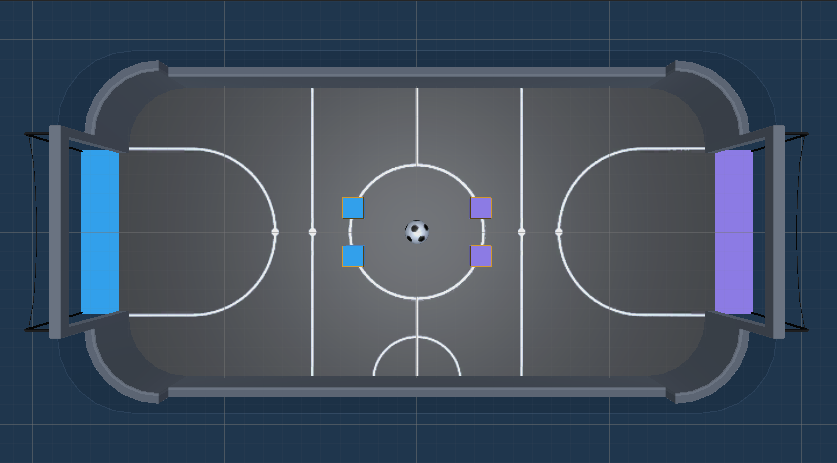
\includegraphics[width=0.7\linewidth]{figures/soccer_field.png}
    \caption{A screenshot of the soccer field taken from the Unity editor}
    \label{fig:soccer_field}
\end{figure}

\noindent
%Overview with image
Here I will lay out the workings of the environment I opted to use, explain the integration with with python, and go over some of the code crucial to its function. This section describes the baseline  modified "Soccer" environment. "Soccer" is the name used in the ML-Agents toolkit. I work with variations on it in \ref{sec:tr:variations}, they all depend on this baseline. The environment I use to train the agent is a simplified version of a game of soccer. 

\subsection{Suitability for my Work}\label{subsec:ip:environment:suitabilty}
At the beginning of this thesis I was faced with the decision whether I should use a preexisting environment or create my own. I opted to make use of an already existing one since this was more in line with my lead question, which asks how an agent is trained. I chose this specific environment because it presents a decent balance between complexity, likelyhood of successful training, intrigue and extensabilty. Due to its extensabilty i could also train and test agents on variations of it, thereby having a measure of how adaptable it is. Further after the modifications I made to the environment it now also offers continuous control to the agent, this presents an interesting challenge, relevant to real world task, where input is seldom binary.

\subsection{Specifics of Operation}\label{subsec:ip:environment:implementation}
The baseline environment is in function mostly identical to the "Soccer" example environment provided by the Unity ML-Agents toolkit. Here I will go over it's sequence of operation, it's specification, and state all the changes I made to it in order to make it suit my work better. The game of soccer takes place on a bounded field and has four players, distributed across two teams. All Each Player is its own Agent, they all act on the same policy and all produce trajectories for it's training. Thereby the policy is trained in play against itself. 

\newpage

\subsubsection{Observations}\label{subsubsec:ip:environment:impl:observations}

\begin{figure}[H]
    \centering
    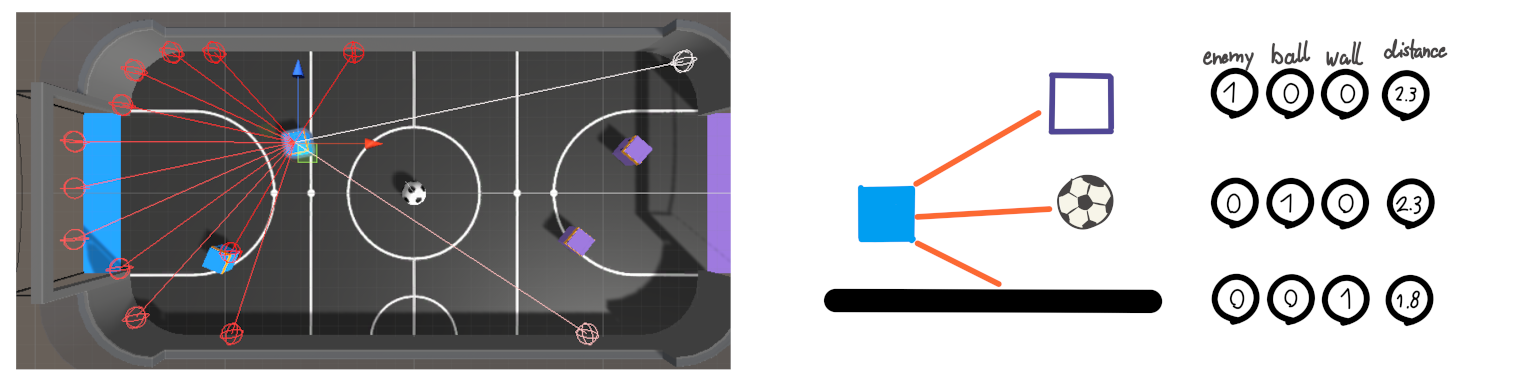
\includegraphics[width=1\linewidth]{figures/ray_sensor.png}
    \caption{Caption}
    \label{fig:ray_sensor}
\end{figure}
\noindent
The "Soccer" example environment uses "Ray Perception Sensors" to create an observation for the agent. A ray perception sensor works by casting a number of rays spread out through a predefined field of view. Along each of these rays a sphere is slid, starting at the agents position and stopping on collision with an object. Each ray contains information about the distance to the object it hit, and its type. The types are predefined, in the case of "Soccer" they are "wall", "enemy", "teammate", "team goal", "enemy goal" and "ball". To the agent a vector is then passed, consisting of the distance to the object the ray struck, as well as its one-hot encoded type. The above figure illustrates how one-hot encoding works and how the observation vectors looks for each ray. The observation vectors are then concatenated to form one single vector, this is then used as the input layer of my policy network. One-hot encoding is commonly used in machine learning where a type information needs to be passed as input, this way separate trainable weights are present for each category. The episode ends if either a goal is score, or a maximum of $600$ time steps pass.

\subsubsection{Episode Start}\label{subsubsec:ip:environment:impl:start}
\textcolor{red}{\textbf{WRITE IN CHAPTER \ref{chap:training} ABOUT THE RANDOMIZATION}}

\subsubsection{Actions}\label{subsubsec:ip:environment:impl:actions}
The environment takes continuous action input from the agent. This was not the case in the example environment provided. Three single precision floating point values are expected, they represent forward, lateral, and rotational movement respectively. This is the \code{C\#} code I use to move the agent:

\begin{lstlisting}[basicstyle=\footnotesize]
public void MoveAgent(ActionSegment<float> act) {
    m_KickPower = 0f;

    float longitudinalAxis = Convert.ToSingle(System.Math.Tanh(act[0])) * m_ForwardSpeed;
    float lateralAxis = Convert.ToSingle(System.Math.Tanh(act[1])) * m_LateralSpeed;
    float rotationalAxis = Convert.ToSingle(System.Math.Tanh(act[2]));

    Transform transformTMP;
    (transformTMP = transform).Rotate(transform.up, rotationalAxis * 6.5f);
    agentRb.AddForce(
        (transformTMP.forward * longitudinalAxis +
         transformTMP.right * lateralAxis)
        * m_SoccerSettings.agentRunSpeed,
        ForceMode.VelocityChange);
}
\end{lstlisting}
\noindent
As visible here, I use the scaled arctangent of the action values received. This is to prevent unexpected behaviour which might result when the values the agent selects are too large. The scaling values for forward and lateral speed are the same as the ones used in the "Soccer" example environment. They are \code{m\_LateralSpeed \= 0.3f;} and \code{m\_ForwardSpeed \= 1.0f;}. The \code{agentRunSpeed} is \code{2.0f}.

%Continuous Action Space
%tanh to bind 
\subsubsection{Rewards}\label{subsubsec:ip:environment:impl:rewards}
In the baseline environment I use the rewards provided by the ML-Agents toolkit. The only rewards given to the agent over the course of the episode are on collision with the ball, in which case a reward of \code{0.2} is given, and the end of the episode. This reward is \code{1.0 + timePenalty} if the episode terminated because the agents team managed to score a goal, if the episode ended in a draw or the agent's team lost it is \code{-1.0}. The \code{timePenalty} is accumulated at every time step according to \code{timePenalty -= m_Existential;}, with \code{m_Existential} being the inverse of the maximum episode length. If there was no time penalty it might me more advantageous for the agents to only repeatedly hit the ball instead of scoring goals.
%perform same action for 10 steps
%quit after n steps
%random agent heurisitc 
%Some Code Snippets 
\subsection{Communication with Policy in Python}\label{subsec:ip:environment:communication_python}
One of the reasons the ML-Agents toolkit is particularly appealing is because it allows for extensive control of the environment in Python. The toolkit provides a Python side API with the \code{mlagents} and \code{mlagents_envs} modules. The figure below, taken from \cite[p. 12]{juliani2020unity}, illustrates this interface.

\begin{figure}[H]
    \centering
    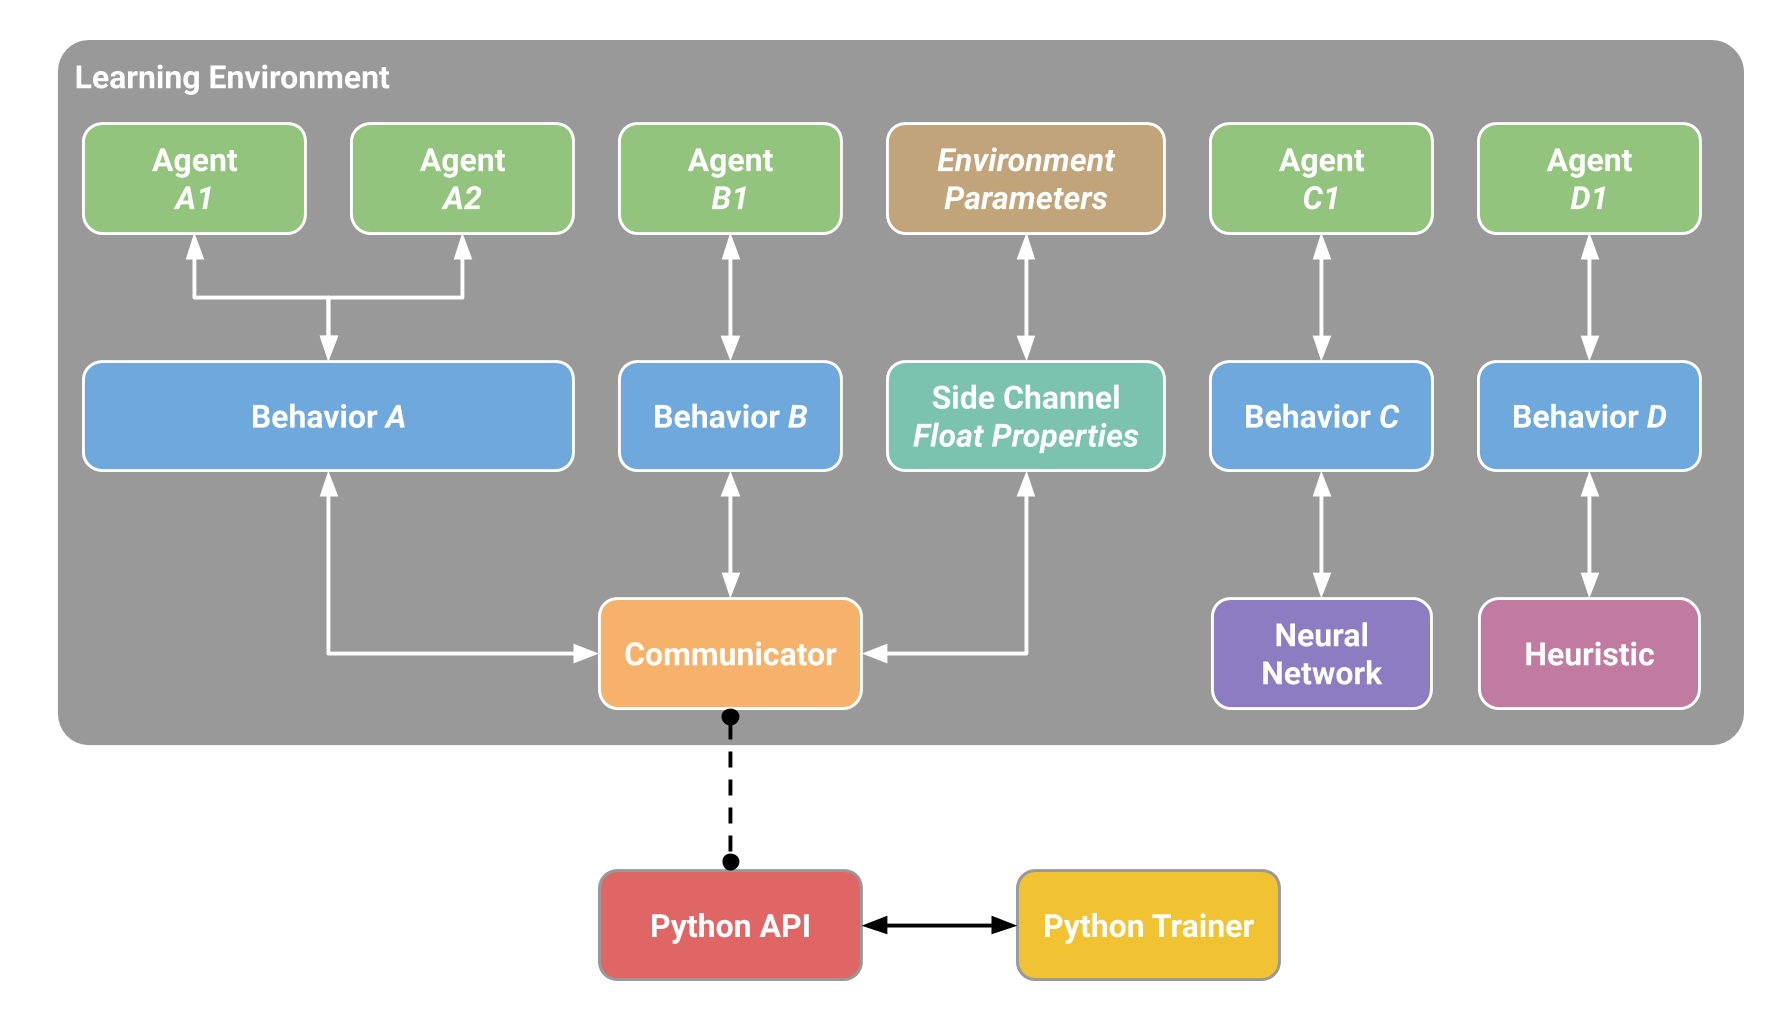
\includegraphics[width=0.75\linewidth]{figures/ml_agents_python_communicator.png}
    \caption{Caption}
    \label{fig:python_communicator}
\end{figure}

\noindent
Through the Python API it is possible to train multiple agents, with possibly differing Behaviours (formally, each of these behaviours would represent a different environment because the observations and actions, as well as the underlying environment functions differ from those of other behaviours, they are effectively a different MDP, see section \ref{sec:MDP}), and even to have yet other agents running on inference (acting on policies which are not being updated, here "Neural Network") or heuristics. This allows for tremendous flexibility not only in training but also allowed me to more fully consider lead question which also pertains to observation, action and reward design. On the Python side of the ML-Agents training framework there exists aside from various other classes which I will briefly cover in section \ref{sec:ip:agent_implementation}, the \code{UnityEnvironment} class. Instantiating it launches, and creates an interface with a Unity executable \cite[p. 13]{juliani2020unity}. From an instance of \code{UnityEnvironment} information about the observation and action type and size can be obtained. During training and evaluation observations, actions, stepping of the environment, and restarting episodes are all handled through this class's members.

\section{The Agent Implementation}\label{sec:ip:agent_implementation}
\subsection{The Agent Policy Network}\label{subsec:ip:agent:network}
%Some Network Code
%Structure 
%Why I chose that structure
\subsection{The Parameter Update Function}\label{subsec:ip:agent:training_func}
%S
\subsection{Efficient Computation of Returns}\label{subsec:ip:agnet:return_calc}
\subsection{Caching experience, delayed Training}\label{subsec:ip:agent:archive}
\section{End-to-End Training and Evaluation}\label{sec:ip:training_testing}
\subsection{The Training Loop}\label{subsec:ip:tt:training_loop}
\subsection{Evaluation}\label{subsec:ip:tt:eval}

